%%%%%%%%%%%%%%%%%%%%%%%%%%%%%%%%%%%%%%%%%%%%%%%%%%%%%%%%%%%%%%%%%%%%%%
\begin{frame}[fragile]\frametitle{}
\begin{center}
{\Large Sorting}
\end{center}

\end{frame}

%%%%%%%%%%%%%%%%%%%%%%%%%%%%%%%%%%%%%%%%%%%%%%%%%%%%%%%%%%%%%%%%%%%%%%
\begin{frame}
	\frametitle{BogoSort}
			The easiest form of sorting: Just try all permutations of the list.
		
Time complexity?:
			\begin{itemize}
				\item $\Theta(n)$
				\item $\Theta(n^2)$
				\item $\Theta(2^n)$
				\item $\Theta(n^n)$
				\item $\Theta(n!)$
				\item I don't know
			\end{itemize}
\end{frame}

%%%%%%%%%%%%%%%%%%%%%%%%%%%%%%%%%%%%%%%%%%%%%%%%%%%%%%%%%%%%%%%%%%%%%%
\begin{frame}
	\frametitle{Some questions and answers}
	Some observations and questions.
	\begin{itemize}
		\item The solution space is huge: $n!$ for $n$ items.
			
		\item The use case is not uncommon, so we hope/look for an efficient (polynomial time) algorithm.
			
		\item Humans have a lot of experience sorting items, can we use those strategies?
			
		\item Or are there methods that computers excel at, that would be terrible for humans?
	\end{itemize}

	\begin{itemize}
		\item There are polynomial time algorithms,
			
		\item We can translate our own methods,
		\item But computers can definitely do better.
	\end{itemize}
\end{frame}

%%%%%%%%%%%%%%%%%%%%%%%%%%%%%%%%%%%%%%%%%%%%%%%%%%%%%%%%%%%%%%%%%%%%%%
\begin{frame}
	\frametitle{Use case?}
		What do we use sorting for?
	
Many things!
		\begin{itemize}
			\item Books in the library.
			\item Exams for an exam review.
			\item Closest pair of points.
			\item Convex hulls.
			\item Efficient look-ups in lists that do not change.
			\item And many many more (see also later lectures in graph algorithms).
		\end{itemize}	
\end{frame}

%%%%%%%%%%%%%%%%%%%%%%%%%%%%%%%%%%%%%%%%%%%%%%%%%%%%%%%%%%%%%%%%%%%%%%
\begin{frame}[fragile]\frametitle{}
\begin{center}
{\Large Bubble Sort}
\end{center}

\end{frame}


%%%%%%%%%%%%%%%%%%%%%%%%%%%%%%%%%%%%%%%%%%%%%%%%%%%%%%%%%%%%%%%%%%%%%%
\begin{frame}[fragile]
	\frametitle{Bubble sort}
	
Your algorithm:
				\begin{lstlisting}
					While $v_i > v_{i+1}$ for some $i$
						State Switch them around.	
					EndWhile
				\end{lstlisting}
			
			\begin{center}
			\begin{tikzpicture}[scale=0.85, transform shape]
	\only<3>{
		\foreach \x/\val in {0/1,1/20,2/42,3/22,4/17}{
			\node[draw,rectangle, fill=gray!10, minimum size =1cm] (c) at (\x,0) {\val};
		}
	}
	\only<4>{
		\foreach \x/\val/\col in {0/1/green,1/20/green,2/42/black,3/22/black,4/17/black}{
			\node[draw=\col,rectangle, fill=\col!10, minimum size =1cm] (c) at (\x,0) {\val};
		}
	}
	\only<5>{
		\foreach \x/\val/\col in {0/1/black,1/20/green,2/42/green,3/22/black,4/17/black}{
			\node[draw=\col,rectangle, fill=\col!10, minimum size =1cm] (c) at (\x,0) {\val};
		}
	}
	\only<6>{
		\foreach \x/\val/\col in {0/1/black,1/20/black,2/42/red,3/22/red,4/17/black}{
			\node[draw=\col,rectangle, fill=\col!10, minimum size =1cm] (c) at (\x,0) {\val};
		}
	}
	\only<7>{
		\foreach \x/\val/\col in {0/1/black,1/20/black,2/22/green,3/42/green,4/17/black}{
			\node[draw=\col,rectangle, fill=\col!10, minimum size =1cm] (c) at (\x,0) {\val};
		}
	}
	\only<8>{
		\foreach \x/\val/\col in {0/1/black,1/20/black,2/22/black,3/42/red,4/17/red}{
			\node[draw=\col,rectangle, fill=\col!10, minimum size =1cm] (c) at (\x,0) {\val};
		}
	}
	\only<9>{
		\foreach \x/\val/\col in {0/1/black,1/20/black,2/22/black,3/17/green,4/42/green}{
			\node[draw=\col,rectangle, fill=\col!10, minimum size =1cm] (c) at (\x,0) {\val};
		}
	}
	\only<10>{
		\foreach \x/\val/\col in {0/1/green,1/20/green,2/22/black,3/17/black,4/42/black}{
			\node[draw=\col,rectangle, fill=\col!10, minimum size =1cm] (c) at (\x,0) {\val};
		}
	}
	\only<11>{
		\foreach \x/\val/\col in {0/1/black,1/20/green,2/22/green,3/17/black,4/42/black}{
			\node[draw=\col,rectangle, fill=\col!10, minimum size =1cm] (c) at (\x,0) {\val};
		}
	}
	\only<12>{
		\foreach \x/\val/\col in {0/1/black,1/20/black,2/22/red,3/17/red,4/42/black}{
			\node[draw=\col,rectangle, fill=\col!10, minimum size =1cm] (c) at (\x,0) {\val};
		}
	}
	\only<13>{
		\foreach \x/\val/\col in {0/1/black,1/20/black,2/17/green,3/22/green,4/42/black}{
			\node[draw=\col,rectangle, fill=\col!10, minimum size =1cm] (c) at (\x,0) {\val};
		}
	}
	\only<14>{
		\foreach \x/\val/\col in {0/1/black,1/20/black,2/17/black,3/22/green,4/42/green}{
			\node[draw=\col,rectangle, fill=\col!10, minimum size =1cm] (c) at (\x,0) {\val};
		}
	}
	\only<15>{
		\foreach \x/\val/\col in {0/1/green,1/20/green,2/17/black,3/22/black,4/42/black}{
			\node[draw=\col,rectangle, fill=\col!10, minimum size =1cm] (c) at (\x,0) {\val};
		}
	}
	\only<16>{
		\foreach \x/\val/\col in {0/1/black,1/20/red,2/17/red,3/22/black,4/42/black}{
			\node[draw=\col,rectangle, fill=\col!10, minimum size =1cm] (c) at (\x,0) {\val};
		}
	}
	\only<17>{
		\foreach \x/\val/\col in {0/1/black,1/17/green,2/20/green,3/22/black,4/42/black}{
			\node[draw=\col,rectangle, fill=\col!10, minimum size =1cm] (c) at (\x,0) {\val};
		}
	}
	\only<18>{
		\foreach \x/\val/\col in {0/1/black,1/17/black,2/20/green,3/22/green,4/42/black}{
			\node[draw=\col,rectangle, fill=\col!10, minimum size =1cm] (c) at (\x,0) {\val};
		}
	}
	\only<19>{
		\foreach \x/\val/\col in {0/1/black,1/17/black,2/20/black,3/22/green,4/42/green}{
			\node[draw=\col,rectangle, fill=\col!10, minimum size =1cm] (c) at (\x,0) {\val};
		}
	}
	\only<20>{
		\foreach \x/\val/\col in {0/1/green,1/17/green,2/20/black,3/22/black,4/42/black}{
			\node[draw=\col,rectangle, fill=\col!10, minimum size =1cm] (c) at (\x,0) {\val};
		}
	}
	\only<21>{
		\foreach \x/\val/\col in {0/1/black,1/17/green,2/20/green,3/22/black,4/42/black}{
			\node[draw=\col,rectangle, fill=\col!10, minimum size =1cm] (c) at (\x,0) {\val};
		}
	}
	\only<22>{
		\foreach \x/\val/\col in {0/1/black,1/17/black,2/20/green,3/22/green,4/42/black}{
			\node[draw=\col,rectangle, fill=\col!10, minimum size =1cm] (c) at (\x,0) {\val};
		}
	}
	\only<23->{
		\foreach \x/\val/\col in {0/1/black,1/17/black,2/20/black,3/22/green,4/42/green}{
			\node[draw=\col,rectangle, fill=\col!10, minimum size =1cm] (c) at (\x,0) {\val};
		}
	}
\end{tikzpicture}

			\end{center}

				So how many inversions can there be?
				\begin{itemize}
					\item $\Theta(n)$
					\item $\Theta(n^2)$
					\item $\Theta(n^n)$
					\item $\Theta(n!)$
				\end{itemize}
\end{frame}

%%%%%%%%%%%%%%%%%%%%%%%%%%%%%%%%%%%%%%%%%%%%%%%%%%%%%%%%%%%%%%%%%%%%%%
\begin{frame}
	\frametitle{The number of inversions}

		Consider a list in reverse order:
		\begin{itemize}
			\item The first element is wrong compared to all others: $n-1$ inversions.
		
			\item The second is also wrong with all the ones that come after it: $n-2$ extra inversions.
			\item \ldots
		
			\item The one-but last one is also wrong with the last one: $1$ inversion
		
			\item So $\Theta(n^2)$ inversion!
		\end{itemize}
\end{frame}

%%%%%%%%%%%%%%%%%%%%%%%%%%%%%%%%%%%%%%%%%%%%%%%%%%%%%%%%%%%%%%%%%%%%%%
\begin{frame}
	\frametitle{To summarise in code}
	\begin{columns}[T]
		\column{0.565\textwidth}
	\lstinputlisting{src/bs.py}
		\column{0.455\textwidth}
Pros and Cons?:
			What are the pros and cons of bubblesort? Hint: remember I told you it was slow!
	\end{columns}
\end{frame}

%%%%%%%%%%%%%%%%%%%%%%%%%%%%%%%%%%%%%%%%%%%%%%%%%%%%%%%%%%%%%%%%%%%%%%
\begin{frame}
	\frametitle{Bubblesort: Pros and Cons}

			While there are inversions: fix them.
Pros:
			\begin{itemize}
				\item Great in a distributed setting, with autonomous agents (like students in a lecture hall).
				\item When implemented as: ``continue while there are inversion'' can terminate after one iteration over a
					sorted list! 
				\item Easiest to implement.
			\end{itemize}


Cons:
			\begin{itemize}
				\item Terribly slow! (Often still slower than other $\Theta(n^2)$ algorithms we will see later)
			\end{itemize}
\end{frame}

%%%%%%%%%%%%%%%%%%%%%%%%%%%%%%%%%%%%%%%%%%%%%%%%%%%%%%%%%%%%%%%%%%%%%%
\begin{frame}[fragile]\frametitle{}
\begin{center}
{\Large Bucket Sort}
\end{center}

\end{frame}

%%%%%%%%%%%%%%%%%%%%%%%%%%%%%%%%%%%%%%%%%%%%%%%%%%%%%%%%%%%%%%%%%%%%%%
\begin{frame}
	\frametitle{Bucket Sort}
The Stephen Tatlock algorithm\dots 

			\begin{itemize}
				\item Sort the items into buckets (e.g. based on first letter of last name).
					
				\item Sort every bucket.
					
				\item Concatenate all buckets together.
			\end{itemize}
		

			Why should we use this?
		
			\begin{itemize}
				\item Great for parallelisation!
				\item Great for humans (sorting a bucket can be done using a different algorithm, everyone can pick their own
					favourite).
				\item Average case analysis is interesting for this algorithm (and gets us to something close to linear time for
					average case).
			\end{itemize}
\end{frame}

%%%%%%%%%%%%%%%%%%%%%%%%%%%%%%%%%%%%%%%%%%%%%%%%%%%%%%%%%%%%%%%%%%%%%%
\begin{frame}[fragile]\frametitle{}
\begin{center}
{\Large Selection Sort}
\end{center}

\end{frame}

%%%%%%%%%%%%%%%%%%%%%%%%%%%%%%%%%%%%%%%%%%%%%%%%%%%%%%%%%%%%%%%%%%%%%%
\begin{frame}
	\frametitle{Selection Sort}
			\begin{itemize}
				\item The smallest of variations \ldots
				\item Rather than shifting every element to it's correct place\dots
				\item We instead repeatedly search for the smallest element and put it at the end of our sorted list/sorted part.
			\end{itemize}
				
	\begin{center}
	\section{Selection Sort}
\label{sec:selection_sort}

\begin{frame}
	\frametitle{Selection Sort}
		\begin{block}{The smallest of variations...}
			Rather than shifting every element to it's correct place\dots\\
			\pause
			We instead repeatedly search for the smallest element and put it at the end of our sorted list/sorted part.
		\end{block}	
	\begin{center}
	\section{Selection Sort}
\label{sec:selection_sort}

\begin{frame}
	\frametitle{Selection Sort}
		\begin{block}{The smallest of variations...}
			Rather than shifting every element to it's correct place\dots\\
			\pause
			We instead repeatedly search for the smallest element and put it at the end of our sorted list/sorted part.
		\end{block}	
	\begin{center}
	\section{Selection Sort}
\label{sec:selection_sort}

\begin{frame}
	\frametitle{Selection Sort}
		\begin{block}{The smallest of variations...}
			Rather than shifting every element to it's correct place\dots\\
			\pause
			We instead repeatedly search for the smallest element and put it at the end of our sorted list/sorted part.
		\end{block}	
	\begin{center}
	\input{figures/tikz/selectionsort.tex}
	\end{center}
\end{frame}

\begin{frame}
	\frametitle{Implementation}
	\begin{exampleblock}{Time Complexity}
		Still $\Theta(n^2)$ as we need to find the minimum $O(n)$ times, which takes $O(n)$ time.
		\end{exampleblock}	
	\begin{alertblock}{See next week's homework}
		You will tell me next week ;)
	\end{alertblock}	
\end{frame}

\begin{frame}
	\frametitle{In-place sorting algorithms}
	\framesubtitle{I'm not going anywhere!}

	\begin{itemize}
		\item The sorting algorithms we have seen so-far are \alert{in-place} sorting algorithms.
			\pause
		\item They take a list and modify that list to become sorted.
			\pause
		\item Of course we can also make them not in-place, by first making a copy of the list and sorting that.
			\pause
		\item But after the break (when we discuss merge sort) we will see an example of an algorithm that is easier to make
			not in-place.
	\end{itemize}
\end{frame}



	\end{center}
\end{frame}

\begin{frame}
	\frametitle{Implementation}
	\begin{exampleblock}{Time Complexity}
		Still $\Theta(n^2)$ as we need to find the minimum $O(n)$ times, which takes $O(n)$ time.
		\end{exampleblock}	
	\begin{alertblock}{See next week's homework}
		You will tell me next week ;)
	\end{alertblock}	
\end{frame}

\begin{frame}
	\frametitle{In-place sorting algorithms}
	\framesubtitle{I'm not going anywhere!}

	\begin{itemize}
		\item The sorting algorithms we have seen so-far are \alert{in-place} sorting algorithms.
			\pause
		\item They take a list and modify that list to become sorted.
			\pause
		\item Of course we can also make them not in-place, by first making a copy of the list and sorting that.
			\pause
		\item But after the break (when we discuss merge sort) we will see an example of an algorithm that is easier to make
			not in-place.
	\end{itemize}
\end{frame}



	\end{center}
\end{frame}

\begin{frame}
	\frametitle{Implementation}
	\begin{exampleblock}{Time Complexity}
		Still $\Theta(n^2)$ as we need to find the minimum $O(n)$ times, which takes $O(n)$ time.
		\end{exampleblock}	
	\begin{alertblock}{See next week's homework}
		You will tell me next week ;)
	\end{alertblock}	
\end{frame}

\begin{frame}
	\frametitle{In-place sorting algorithms}
	\framesubtitle{I'm not going anywhere!}

	\begin{itemize}
		\item The sorting algorithms we have seen so-far are \alert{in-place} sorting algorithms.
			\pause
		\item They take a list and modify that list to become sorted.
			\pause
		\item Of course we can also make them not in-place, by first making a copy of the list and sorting that.
			\pause
		\item But after the break (when we discuss merge sort) we will see an example of an algorithm that is easier to make
			not in-place.
	\end{itemize}
\end{frame}



	\end{center}
\end{frame}

%%%%%%%%%%%%%%%%%%%%%%%%%%%%%%%%%%%%%%%%%%%%%%%%%%%%%%%%%%%%%%%%%%%%%%
\begin{frame}
	\frametitle{Implementation}
Time Complexity: 		Still $\Theta(n^2)$ as we need to find the minimum $O(n)$ times, which takes $O(n)$ time.
	
\end{frame}

%%%%%%%%%%%%%%%%%%%%%%%%%%%%%%%%%%%%%%%%%%%%%%%%%%%%%%%%%%%%%%%%%%%%%%

\begin{frame}
	\frametitle{In-place sorting algorithms}

	\begin{itemize}
		\item The sorting algorithms we have seen so-far are \alert{in-place} sorting algorithms.
			
		\item They take a list and modify that list to become sorted.
			
		\item Of course we can also make them not in-place, by first making a copy of the list and sorting that.
			
		\item But after the break (when we discuss merge sort) we will see an example of an algorithm that is easier to make
			not in-place.
	\end{itemize}
\end{frame}

%%%%%%%%%%%%%%%%%%%%%%%%%%%%%%%%%%%%%%%%%%%%%%%%%%%%%%%%%%%%%%%%%%%%%%
\begin{frame}[fragile]\frametitle{}
\begin{center}
{\Large Insertion Sort}
\end{center}

\end{frame}

%%%%%%%%%%%%%%%%%%%%%%%%%%%%%%%%%%%%%%%%%%%%%%%%%%%%%%%%%%%%%%%%%%%%%%
\begin{frame}
	\frametitle{Insertion Sort}

			The main idea:
			\begin{itemize}
				\item We build the list, step by step.
					
				\item We keep our intermediate result sorted.
					
				\item At every step, we insert the next element into the right place.
					
				\item This means we need to shift over (worst-case) $n$ elements for every element we insert...
					
				\item So in total $\Theta(n^2)$ time.
			\end{itemize}

\end{frame}

%%%%%%%%%%%%%%%%%%%%%%%%%%%%%%%%%%%%%%%%%%%%%%%%%%%%%%%%%%%%%%%%%%%%%%
\begin{frame}[fragile]
	\frametitle{Insertion Sort}
	
	\begin{lstlisting}
		State $i gets 1$ Comment {The first element forms a sorted list on it's own}
		
		While $i < \texttt{len}(l)$
		State $j gets i$
		
		While $j > 0$ and $v_{j-1} < v_{j}$ 
			State swap $v_j$ and $v_{j-1}$	
			State $j gets j -1$
		EndWhile
		
		State $i gets i+1$
		EndWhile
	\end{lstlisting}
	
	\begin{center}
	\section{Insertion Sort}
\label{sec:insertion_sort}

\begin{frame}
	\frametitle{Insertion sort}
	\begin{center}
		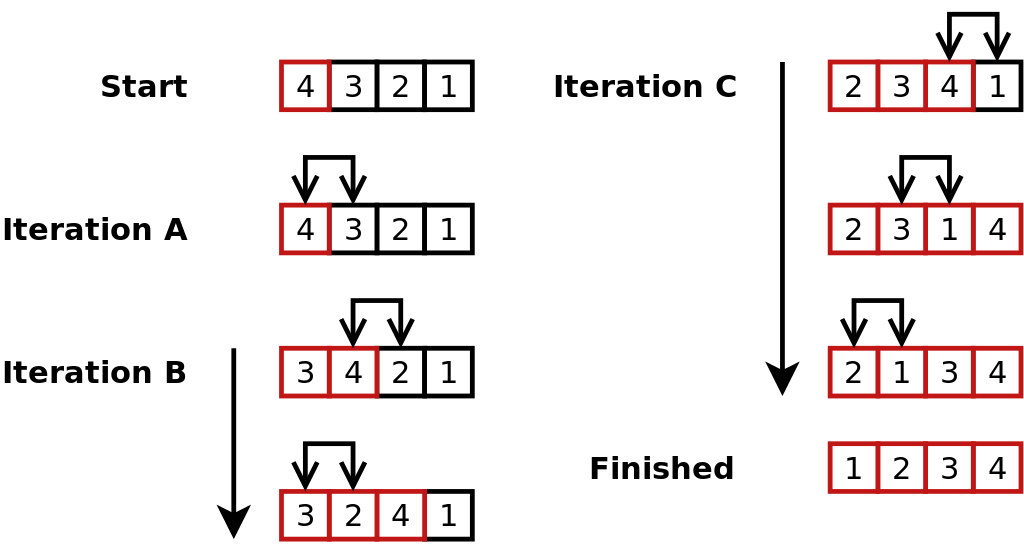
\includegraphics[width=0.8\textwidth]{figures/insertionsort.png}\\
		\hspace*{15pt}\hbox{\scriptsize Image By:\thinspace{\itshape MrDrBob}}
		% https://commons.wikimedia.org/wiki/File:Insertion-sort.svg
	\end{center}
\end{frame}

\begin{frame}
	\frametitle{Insertion Sort}
	\framesubtitle{How does that work?}
		\begin{block}{Insertion Sort}
			The main idea:
			\begin{itemize}
				\item We build the list, step by step.
					\pause
				\item We keep our intermediate result sorted.
					\pause
				\item At every step, we insert the next element into the right place.
					\pause
				\item This means we need to shift over (worst-case) $n$ elements for every element we insert...
					\pause
				\item So in total $\Theta(n^2)$ time.
			\end{itemize}
		\end{block}
\end{frame}

\begin{frame}
	\frametitle{Insertion Sort}
	\begin{algorithmic}
		\State $i \gets 1$ \Comment{The first element forms a sorted list on it's own}
		\pause
		\While{$i < \texttt{len}(l)$}
		\State $j \gets i$
		\pause
		\While{$j > 0$ and $v_{j-1} < v_{j}$}
			\State swap $v_j$ and $v_{j-1}$	
			\State $j \gets j -1$
		\EndWhile
		\pause
		\State $i \gets i+1$
		\EndWhile
	\end{algorithmic}
	\pause
	\begin{center}
	\section{Insertion Sort}
\label{sec:insertion_sort}

\begin{frame}
	\frametitle{Insertion sort}
	\begin{center}
		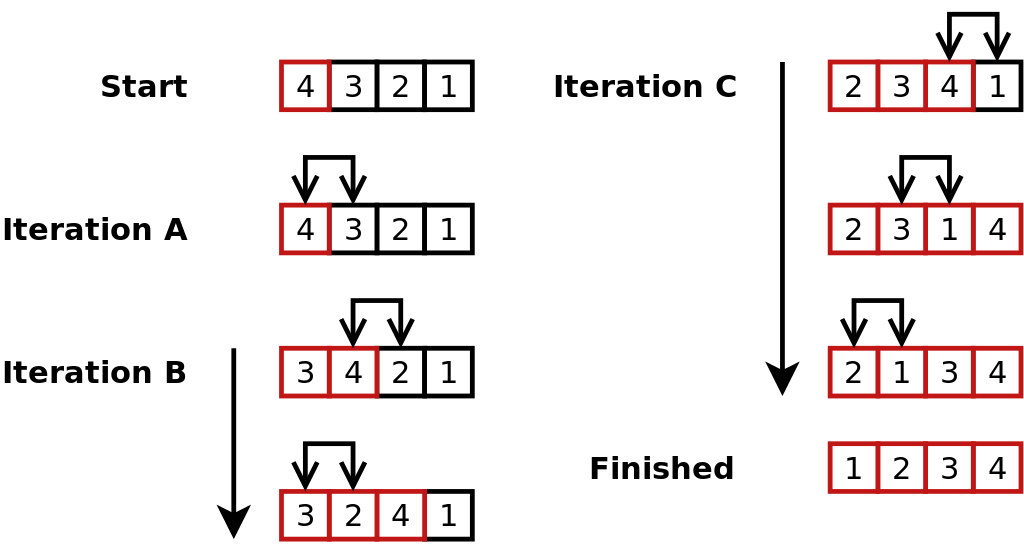
\includegraphics[width=0.8\textwidth]{figures/insertionsort.png}\\
		\hspace*{15pt}\hbox{\scriptsize Image By:\thinspace{\itshape MrDrBob}}
		% https://commons.wikimedia.org/wiki/File:Insertion-sort.svg
	\end{center}
\end{frame}

\begin{frame}
	\frametitle{Insertion Sort}
	\framesubtitle{How does that work?}
		\begin{block}{Insertion Sort}
			The main idea:
			\begin{itemize}
				\item We build the list, step by step.
					\pause
				\item We keep our intermediate result sorted.
					\pause
				\item At every step, we insert the next element into the right place.
					\pause
				\item This means we need to shift over (worst-case) $n$ elements for every element we insert...
					\pause
				\item So in total $\Theta(n^2)$ time.
			\end{itemize}
		\end{block}
\end{frame}

\begin{frame}
	\frametitle{Insertion Sort}
	\begin{algorithmic}
		\State $i \gets 1$ \Comment{The first element forms a sorted list on it's own}
		\pause
		\While{$i < \texttt{len}(l)$}
		\State $j \gets i$
		\pause
		\While{$j > 0$ and $v_{j-1} < v_{j}$}
			\State swap $v_j$ and $v_{j-1}$	
			\State $j \gets j -1$
		\EndWhile
		\pause
		\State $i \gets i+1$
		\EndWhile
	\end{algorithmic}
	\pause
	\begin{center}
	\section{Insertion Sort}
\label{sec:insertion_sort}

\begin{frame}
	\frametitle{Insertion sort}
	\begin{center}
		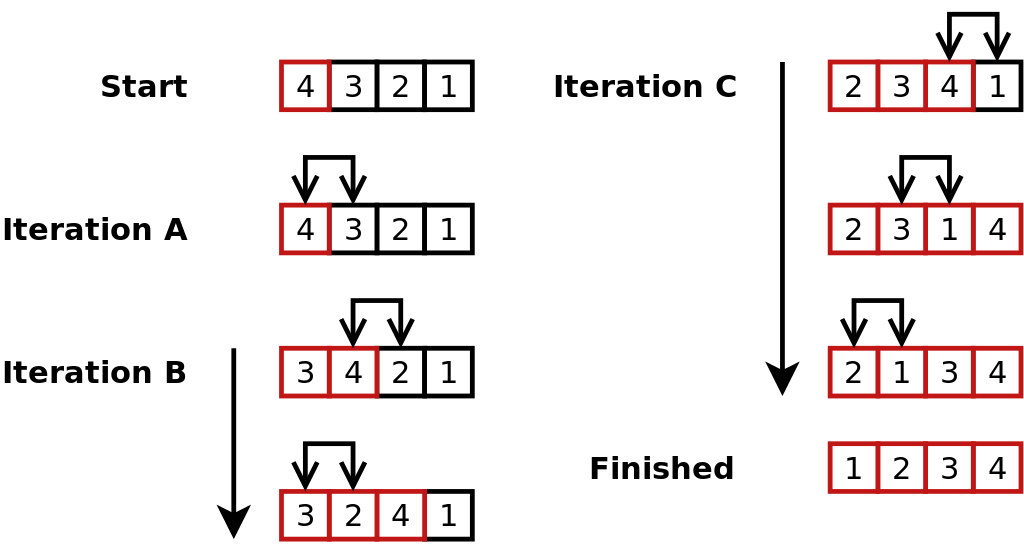
\includegraphics[width=0.8\textwidth]{figures/insertionsort.png}\\
		\hspace*{15pt}\hbox{\scriptsize Image By:\thinspace{\itshape MrDrBob}}
		% https://commons.wikimedia.org/wiki/File:Insertion-sort.svg
	\end{center}
\end{frame}

\begin{frame}
	\frametitle{Insertion Sort}
	\framesubtitle{How does that work?}
		\begin{block}{Insertion Sort}
			The main idea:
			\begin{itemize}
				\item We build the list, step by step.
					\pause
				\item We keep our intermediate result sorted.
					\pause
				\item At every step, we insert the next element into the right place.
					\pause
				\item This means we need to shift over (worst-case) $n$ elements for every element we insert...
					\pause
				\item So in total $\Theta(n^2)$ time.
			\end{itemize}
		\end{block}
\end{frame}

\begin{frame}
	\frametitle{Insertion Sort}
	\begin{algorithmic}
		\State $i \gets 1$ \Comment{The first element forms a sorted list on it's own}
		\pause
		\While{$i < \texttt{len}(l)$}
		\State $j \gets i$
		\pause
		\While{$j > 0$ and $v_{j-1} < v_{j}$}
			\State swap $v_j$ and $v_{j-1}$	
			\State $j \gets j -1$
		\EndWhile
		\pause
		\State $i \gets i+1$
		\EndWhile
	\end{algorithmic}
	\pause
	\begin{center}
	\input{figures/tikz/insertionsort.tex}
	\end{center}
\end{frame}

\begin{frame}
	\frametitle{Would you like some sausages with your cheese?}
	\begin{columns}
		\column{0.455\textwidth}
		\begin{algorithmic}
			\State $i \gets 1$ 
			\While{$i < \texttt{len}(l)$}
			\State $j \gets i$
			\While{$j > 0$ and $v_j < v_{j-1}$}
			\State swap $v_j$ and $v_{j-1}$	
			\State $j \gets j -1$
			\EndWhile
			\State $i \gets i+1$
			\EndWhile
		\end{algorithmic}
		\column{0.455\textwidth}
		\begin{questionblock}{Run time}
			What instance of a list would give the worst performance here?	
		\end{questionblock}
		\pause
		\begin{answerblock}{Again!?}
			Once again it is the reverse list, where every item needs to be moved to the front requiring most swaps.
		\end{answerblock}
		\pause
			\begin{block}{So...}
				The run time is still $\Theta(n^2)$.
			\end{block}	
	\end{columns}

	
\end{frame}

\begin{frame}
	\frametitle{Implementation to summarise}
	
		\begin{alertblock}{See you tomorrow!}
			We will implement this tomorrow :)
		\end{alertblock}	
\end{frame}

\begin{frame}
	\frametitle{Insertion Sort: Pros and Cons}
		\begin{block}{Insertion Sort}
			Repeatedly insert the next item in the correct place in a sorted list.
		\end{block}	
		\begin{exampleblock}{Pros}
			\begin{itemize}
				\item `Easy' algorithm to implement.
				\item Good performance for an $O(n^2)$ algorithm.
			\end{itemize}
		\end{exampleblock}	
		\begin{alertblock}{Cons}
			\begin{itemize}
				\item Still not as fast as comparison-based sorting algorithms can be.
			\end{itemize}
		\end{alertblock}	
	
\end{frame}

	\end{center}
\end{frame}

\begin{frame}
	\frametitle{Would you like some sausages with your cheese?}
	\begin{columns}
		\column{0.455\textwidth}
		\begin{algorithmic}
			\State $i \gets 1$ 
			\While{$i < \texttt{len}(l)$}
			\State $j \gets i$
			\While{$j > 0$ and $v_j < v_{j-1}$}
			\State swap $v_j$ and $v_{j-1}$	
			\State $j \gets j -1$
			\EndWhile
			\State $i \gets i+1$
			\EndWhile
		\end{algorithmic}
		\column{0.455\textwidth}
		\begin{questionblock}{Run time}
			What instance of a list would give the worst performance here?	
		\end{questionblock}
		\pause
		\begin{answerblock}{Again!?}
			Once again it is the reverse list, where every item needs to be moved to the front requiring most swaps.
		\end{answerblock}
		\pause
			\begin{block}{So...}
				The run time is still $\Theta(n^2)$.
			\end{block}	
	\end{columns}

	
\end{frame}

\begin{frame}
	\frametitle{Implementation to summarise}
	
		\begin{alertblock}{See you tomorrow!}
			We will implement this tomorrow :)
		\end{alertblock}	
\end{frame}

\begin{frame}
	\frametitle{Insertion Sort: Pros and Cons}
		\begin{block}{Insertion Sort}
			Repeatedly insert the next item in the correct place in a sorted list.
		\end{block}	
		\begin{exampleblock}{Pros}
			\begin{itemize}
				\item `Easy' algorithm to implement.
				\item Good performance for an $O(n^2)$ algorithm.
			\end{itemize}
		\end{exampleblock}	
		\begin{alertblock}{Cons}
			\begin{itemize}
				\item Still not as fast as comparison-based sorting algorithms can be.
			\end{itemize}
		\end{alertblock}	
	
\end{frame}

	\end{center}
\end{frame}

\begin{frame}
	\frametitle{Would you like some sausages with your cheese?}
	\begin{columns}
		\column{0.455\textwidth}
		\begin{algorithmic}
			\State $i \gets 1$ 
			\While{$i < \texttt{len}(l)$}
			\State $j \gets i$
			\While{$j > 0$ and $v_j < v_{j-1}$}
			\State swap $v_j$ and $v_{j-1}$	
			\State $j \gets j -1$
			\EndWhile
			\State $i \gets i+1$
			\EndWhile
		\end{algorithmic}
		\column{0.455\textwidth}
		\begin{questionblock}{Run time}
			What instance of a list would give the worst performance here?	
		\end{questionblock}
		\pause
		\begin{answerblock}{Again!?}
			Once again it is the reverse list, where every item needs to be moved to the front requiring most swaps.
		\end{answerblock}
		\pause
			\begin{block}{So...}
				The run time is still $\Theta(n^2)$.
			\end{block}	
	\end{columns}

	
\end{frame}

\begin{frame}
	\frametitle{Implementation to summarise}
	
		\begin{alertblock}{See you tomorrow!}
			We will implement this tomorrow :)
		\end{alertblock}	
\end{frame}

\begin{frame}
	\frametitle{Insertion Sort: Pros and Cons}
		\begin{block}{Insertion Sort}
			Repeatedly insert the next item in the correct place in a sorted list.
		\end{block}	
		\begin{exampleblock}{Pros}
			\begin{itemize}
				\item `Easy' algorithm to implement.
				\item Good performance for an $O(n^2)$ algorithm.
			\end{itemize}
		\end{exampleblock}	
		\begin{alertblock}{Cons}
			\begin{itemize}
				\item Still not as fast as comparison-based sorting algorithms can be.
			\end{itemize}
		\end{alertblock}	
	
\end{frame}

	\end{center}
\end{frame}

%%%%%%%%%%%%%%%%%%%%%%%%%%%%%%%%%%%%%%%%%%%%%%%%%%%%%%%%%%%%%%%%%%%%%%
\begin{frame}[fragile]
	\frametitle{Would you like some sausages with your cheese?}
	
	\begin{columns}[T]
		\column{0.455\textwidth}
		\begin{lstlisting}
			State $i \gets 1$ 
			While $i < \texttt{len}(l)$
			State $j \gets i$
			While $j > 0$ and $v_j < v_{j-1}$
			State swap $v_j$ and $v_{j-1}$	
			State $j \gets j -1$
			EndWhile
			State $i \gets i+1$
			EndWhile
		\end{lstlisting}
		\column{0.455\textwidth}
			\begin{itemize}
				\item Run time:		What instance of a list would give the worst performance here?	
				\item Once again it is the reverse list, where every item needs to be moved to the front requiring most swaps.
				\item The run time is still $\Theta(n^2)$.
			\end{itemize}	
	\end{columns}
\end{frame}

%%%%%%%%%%%%%%%%%%%%%%%%%%%%%%%%%%%%%%%%%%%%%%%%%%%%%%%%%%%%%%%%%%%%%%
\begin{frame}
	\frametitle{Insertion Sort: Pros and Cons}
			\begin{itemize}
				\item Insertion Sort:	Repeatedly insert the next item in the correct place in a sorted list.
				\item Pros:
			\begin{itemize}
				\item `Easy' algorithm to implement.
				\item Good performance for an $O(n^2)$ algorithm.
			\end{itemize}
				\item Cons:
			\begin{itemize}
				\item Still not as fast as comparison-based sorting algorithms can be.
			\end{itemize}
		\end{itemize}	
	
\end{frame}

%%%%%%%%%%%%%%%%%%%%%%%%%%%%%%%%%%%%%%%%%%%%%%%%%%%%%%%%%%%%%%%%%%%%%%
\begin{frame}[fragile]\frametitle{}
\begin{center}
{\Large Merge Sort}
\end{center}

\end{frame}

%%%%%%%%%%%%%%%%%%%%%%%%%%%%%%%%%%%%%%%%%%%%%%%%%%%%%%%%%%%%%%%%%%%%%%
\begin{frame}
	\frametitle{Merge Sort}
			\begin{itemize}
				\item A recursive sorting algorithm.
				\item It splits the list into two, sorts each half, then combines the results.

				\item Not great for humans: this algorithm is not the easiest for humans to perform.
				\item Great for computers:	But computers do excellent at it!
	\end{itemize}	
\end{frame}

%%%%%%%%%%%%%%%%%%%%%%%%%%%%%%%%%%%%%%%%%%%%%%%%%%%%%%%%%%%%%%%%%%%%%%
\begin{frame}[fragile]
	\frametitle{The idea}

			The algorithm:
		\begin{lstlisting}
			Function{MergeSort}{xs}
				If{len(xs) $< 2$}	
					State Return xs
				EndIf
			
				State leftHalf $gets$ Call{MergeSort}{the first half of the list}
				State rightHalf $gets$ Call{MergeSort}{the second half of the list}
			
				State result $gets []$, $i gets 0$, $j gets 0$
				While{$i < $ len(leftHalf) and $j < $ len(rightHalf)}
					State\alert{Something goes here}
					State\alert{Update $i$ and $j$ accordingly.}

				:
			EndFunction
		\end{lstlisting}
		

\end{frame}

%%%%%%%%%%%%%%%%%%%%%%%%%%%%%%%%%%%%%%%%%%%%%%%%%%%%%%%%%%%%%%%%%%%%%%
\begin{frame}[fragile]
	\frametitle{The idea}

			The algorithm:
		\begin{lstlisting}
			Function{MergeSort}{xs}
				:

				If{leftHalf[i] $<$ rightHalf[j]}
					State result.append(leftHalf[i]),  $i gets i + 1$
				Else
					State 
					State result.append(rightHalf[j]),  $j gets j + 1$
				EndIf
				State \alert{Something here?}
				While{$i < $ len(leftHalf)}
					State result.append(leftHalf[i]),  $i\gets i + 1$
				EndWhile
				While{$j < $ len(rightHalf)}
					State result.append(rightHalf[j]),  $j\gets j + 1$
				EndWhile
				State Return result
			EndFunction
		\end{lstlisting}
		
\end{frame}

%%%%%%%%%%%%%%%%%%%%%%%%%%%%%%%%%%%%%%%%%%%%%%%%%%%%%%%%%%%%%%%%%%%%%%
\begin{frame}[fragile]
	\frametitle{The idea}

		
			What do we do here?
				\begin{itemize}
					\item Compare leftHalf[0] with rightHalf[0]
					\item Compare leftHalf[i] with rightHalf[0]
					\item Compare leftHalf[0] with rightHalf[j]
					\item Compare leftHalf[i] with rightHalf[j]
				\end{itemize}
				What do we do here?
				\begin{itemize}
					\item Nothing, we're done
					\item Empty the remainder of the left half, then the right half.
					\item Empty the remainder of the right half, then the left half.
					\item Only one half can still have items left, empty that one.
				\end{itemize}
				You can see one con:		The algorithm is a bit more involved \ldots
				Is it better?: What is a tight bound on the run time?	Hint: you can use the master theorem!
\end{frame}

%%%%%%%%%%%%%%%%%%%%%%%%%%%%%%%%%%%%%%%%%%%%%%%%%%%%%%%%%%%%%%%%%%%%%%
\begin{frame}
	\frametitle{Merge sort run time}
				\begin{itemize}
					\item $T(0) = T(1) = c_0$ and $T(n) = 2T(n/2) + \Theta(n)$
					\item This gives $n^{\log_2(2)} = n$ leaves, and as $f(n) = \Theta(n)$ this makes this case 2 of the master method
					\item Thus $\Theta(n\log n)$ work! We improved!
					\item Worst-case instance?:
		What would be the worst type of list for this algorithm?
	
					\item There is none
					\item There is no worst-case instance, all of them take $\Theta(n \log n)$ time as we append $n$ items in $\log n$
		recursive calls in the recursion tree.
	\end{itemize}
\end{frame}

%%%%%%%%%%%%%%%%%%%%%%%%%%%%%%%%%%%%%%%%%%%%%%%%%%%%%%%%%%%%%%%%%%%%%%
\begin{frame}
	\frametitle{Merge sort: pros and cons}
	\begin{block}{Merge sort}
			Recursively split the list, sort and merge sorted lists.
		\end{block}	
		\begin{block}{Pros}
			\begin{itemize}
				\item Great in a distributed setting, as it can be parallelised!
				\item Great time complexity! $O(n\log n)$
			\end{itemize}
		\end{block}	
		\begin{block}{Cons}
			\begin{itemize}
				\item A bit harder to implement.
				\item Always takes $O(n \log n)$ even when only two items would have to be switched.
			\end{itemize}
		\end{block}	
\end{frame}

%%%%%%%%%%%%%%%%%%%%%%%%%%%%%%%%%%%%%%%%%%%%%%%%%%%%%%%%%%%%%%%%%%%%%%
\begin{frame}[fragile]\frametitle{}
\begin{center}
{\Large Quick Sort}
\end{center}

\end{frame}

%%%%%%%%%%%%%%%%%%%%%%%%%%%%%%%%%%%%%%%%%%%%%%%%%%%%%%%%%%%%%%%%%%%%%%
\begin{frame}
	\frametitle{Quicksort}
			\begin{itemize}
				\item A recursive sorting algorithm.
				\item It splits the list into two, sorts each half, then combines the results.
				\item That sounds exactly like mergesort!?
	\end{itemize}	
\end{frame}

%%%%%%%%%%%%%%%%%%%%%%%%%%%%%%%%%%%%%%%%%%%%%%%%%%%%%%%%%%%%%%%%%%%%%%
\begin{frame}[fragile]
	\frametitle{The idea}
		\begin{columns}[T]
			\column{0.705\textwidth}
			The algorithm:
		\begin{lstlisting}
			Function{Quicksort}{xs}
				If{len(xs) $< 2$}	
					State Return xs
				EndIf
				
				State pivot $gets$ some element from xs
				State left $gets$ everything smaller than pivot
				State right $gets$ everything larger than pivot
				State leftHalf $gets$ Call{Quicksort}{left}
				State rightHalf $gets$ Call{Quicksort}{right}
				
				State Return \alt<5->{leftHalf + pivot + rightHalf}{\dots}
			EndFunction
		\end{lstlisting}
		
			\column{0.305\textwidth}
			What do we do here?
				\begin{itemize}
					\item Merge the left and right half.
					\item Return left + right
					\item Return left + pivot + right
					\item Return right + pivot + left
				\end{itemize}
	
					What is the time complexity of this?\\
					Or rather, what does the worst case input look like?
		\end{columns}
\end{frame}

%%%%%%%%%%%%%%%%%%%%%%%%%%%%%%%%%%%%%%%%%%%%%%%%%%%%%%%%%%%%%%%%%%%%%%
\begin{frame}
	\frametitle{It depends!}
				\begin{itemize}
					\item Everything stands and falls by the choice of pivot.
					\item The first element:
		What is the worst input if we always take the first element as the pivot?
					\item 
					\begin{itemize}
						\item A sorted list
						\item The reverse of a sorted list
						\item A list that has the first $n/2$ elements sorted ascendingly and the second $n/2$ elements sorted descendingly.
					\end{itemize}
					\item This takes of only $1$ element every time, meaning we need $O(n^2)$ time.	
	\end{itemize}
\end{frame}

%%%%%%%%%%%%%%%%%%%%%%%%%%%%%%%%%%%%%%%%%%%%%%%%%%%%%%%%%%%%%%%%%%%%%%
\begin{frame}
	\frametitle{In practice}
	
Quick Sort in the real world:
			\begin{itemize}
				\item It is the most common sorting algorithm used.
				\item The implementations choose \textit{random} pivots.
					
				\item Worst-case this is still $O(n^2)$ of course.
					
				\item But with some fancy analysis (that we will not go into today, but maybe tomorrow ;)), we can show that
					this is $O(n \log n)$ in expectation (average case if you will).
					
				\item In practice this often outperforms merge sort significantly, especially when we make it in-place.
			\end{itemize}
\end{frame}

%%%%%%%%%%%%%%%%%%%%%%%%%%%%%%%%%%%%%%%%%%%%%%%%%%%%%%%%%%%%%%%%%%%%%%
\begin{frame}
	\frametitle{Quicksort: pros and cons}
			\begin{itemize}
				\item Recursively split the list in smaller and larger elements, sort and combine.
				\item Pros:
			\begin{itemize}
				\item Great time complexity for average case $O(n\log n)$
				\item Simpler to implement (and faster in most cases) than merge sort.
				\item Argument based on authority: the whole world uses it.
			\end{itemize}
				\item Cons:
			\begin{itemize}
				\item Still $O(n^2)$ if we are unlucky in choosing pivots.
			\end{itemize}
		\end{itemize}	
\end{frame}

%%%%%%%%%%%%%%%%%%%%%%%%%%%%%%%%%%%%%%%%%%%%%%%%%%%%%%%%%%%%%%%%%%%%%%
\begin{frame}[fragile]\frametitle{}
\begin{center}
{\Large Sorting Summary}
\end{center}

\end{frame}

%%%%%%%%%%%%%%%%%%%%%%%%%%%%%%%%%%%%%%%%%%%%%%%%%%%%%%%%%%%%%%%%%%%%%%
\begin{frame}
	\frametitle{Summary table}
	\begin{tabular}{r | c | c | c}
		\small
		Sorting method & Time & Main advantage & Main disadvantage \\
		\midrule
		Bubble Sort & $O(n^2)$ & Easy for humans! &  Very very very very slow \\
		Insertion Sort & $O(n^2)$ & Good for small lists &  Still quadratic time \\
		Selection Sort & $O(n^2)$ & Good for small lists &  Still quadratic time \\
		Merge Sort & $O(n \log n)$ & Faster than quadratic! &  Bad on `almost sorted lists' \\
		Quick Sort & $O(n \log n)$\footnote{in expectation} & Faster than merge sort &  Still worst-case quadratic\dots \\
	\end{tabular}
	\begin{itemize}
		\item We can mix Bucket Sort in with all this, by applying it first and then applying it (or one of the others) on
			the different buckets.
		\item Sorting algorithms can be in-place or not.
	\end{itemize}
\end{frame}

%%%%%%%%%%%%%%%%%%%%%%%%%%%%%%%%%%%%%%%%%%%%%%%%%%%%%%%%%%%%%%%%%%%%%%
\begin{frame}
	\frametitle{But wait!}
	
	\begin{itemize}
		\item Stable sorting: Didn't I also mention stable sorting yesterday?
		\item A sorting is stable if: in a list where if $k_i = k_j$ (where $k$ denotes the sorting key,
			e.g. age, or length) and $v_i$ comes for $v_j$ before sorting, then $v_i$ still comes before $v_j$ after sorting.
		\item Check for yourselves:
	\begin{itemize}
		\item Insertion sort is stable!
		\item Merge sort is not!
			\end{itemize}

			\end{itemize}	
\end{frame}